\documentclass[12pt,oneside]{book}

	% History ================================================================
	% 2023.06.03 - Modified from Chase Murray's version
	% ========================================================================

    % STANDARD PACKAGES ======================================================
    \usepackage{datetime}
    \usepackage{graphicx}
    % \usepackage{ctex} % Allow Chinese characters
    \usepackage[utf8]{inputenc}
    \usepackage[american]{babel}
    \usepackage{amssymb}
    \usepackage[intlimits]{amsmath}
    \usepackage{amsfonts}
    \usepackage{amsthm}
    \usepackage{array}
    \usepackage{mdwlist}        
    % \usepackage[labelsep=quad,indention=10pt]{subfig}
    \usepackage{algorithm}
    \usepackage[noend]{algpseudocode}
    \usepackage{lscape}
    \usepackage{rotating} % Allows \begin{sideways} \end{sideways} for vertical table headers.    
    \usepackage{threeparttable} % Allow footnotes in tables.    
    \usepackage{tabularx}
    \usepackage{multirow} % Allow table cells to span multiple rows/cols.
    \usepackage{makecell}
    \usepackage{longtable}
    \usepackage{url} % Allow \url{} and \href{url}{name}
    \usepackage{verbatim}    
    \usepackage{enumerate} % http://www.tex.ac.uk/cgi-bin/texfaq2html?label=enumerate
    \usepackage{color} % Allow colored fonts
    \usepackage[toc,page]{appendix}

    \usepackage{bm}

    \usepackage{tikz}
        \usetikzlibrary{shapes.geometric, arrows}
            \tikzstyle{startstop} = [rectangle, rounded corners, minimum width=3cm, minimum height=1cm,text centered, draw=black]
            \tikzstyle{io} = [trapezium, trapezium left angle=70, trapezium right angle=110, minimum width=3cm, minimum height=1cm, text centered, draw=black]
            \tikzstyle{process} = [rectangle, minimum width=2cm, minimum height=1cm, text centered, draw=black, inner sep=0.1cm]
            \tikzstyle{decision} = [diamond, minimum width=2cm, minimum height=0cm, text centered, draw=black, inner sep=0cm]
            \tikzstyle{arrow} = [thick,->,>=stealth]
            \tikzstyle{branchnode} = [circle, minimum size = 1cm, text centered, draw=black, inner sep=0.1cm]
            \tikzstyle{solidNode} = [circle, minimum size = 0.1cm, fill=black]
            \tikzstyle{link} = [thick, -]
            \tikzstyle{matchedLink} = [decorate, decoration={snake}]
            \tikzstyle{circleNode} = [
                circle, 
                minimum size = 0.7cm, 
                text centered, 
                draw=black, 
                inner sep=0.1cm
            ]
    \usepackage{diagbox}
    \usepackage{lastpage} % \pageref{LastPage} = total number of pages.
    \usepackage{ifthen}        
    \usepackage{setspace} % Allows \singlespacing, \onehalfspacing, \doublespacing 
    \usepackage{listings} % Allows formatting of Python code (and other languages)
    % \usepackage{wrapfig}
    \usepackage[normalem]{ulem} % Allows strikethrough (\sout{text to strike})
    % \usepackage{subfigure}        % Allows subfigs/subfloats


    \usepackage{xcolor,colortbl}    % http://ctan.org/pkg/xcolor
    % \usepackage[table]{xcolor}    % https://tex.stackexchange.com/questions/50349/color-only-a-cell-of-a-table
    
    % Make sure that {color} and {xcolor} are called before mdframed
    \usepackage[framemethod=TikZ]{mdframed}    % Allows colored textbox

    \usepackage{lipsum}                     % Dummy text
    % ========================================================================

    % DEFINE PROGRAMMING FORMAT ++++++++++++++++++++++++++++++++++++++++++++++
        \lstset{language=Python}          % Set your language (you can change the language for each code-block optionally)

        \definecolor{mygreen}{rgb}{0,0.6,0}
        \definecolor{mygray}{rgb}{0.5,0.5,0.5}
        \definecolor{mymauve}{rgb}{0.58,0,0.82}

        \lstset{
          backgroundcolor=\color{gray!05!white},   % choose the background color; you must add \usepackage{color} or \usepackage{xcolor}; should come as last argument
          basicstyle=\ttfamily,                    % the size of the fonts that are used for the code
          breakatwhitespace=false,                 % sets if automatic breaks should only happen at whitespace
          breaklines=true,                         % sets automatic line breaking
          captionpos=t,                            % sets the caption-position to bottom
          commentstyle=\color{black},              % comment style
          deletekeywords={...},                    % if you want to delete keywords from the given language
          escapeinside={\%*}{*)},                  % if you want to add LaTeX within your code
          extendedchars=true,                      % lets you use non-ASCII characters; for 8-bits encodings only, does not work with UTF-8
          frame=single,                               % adds a frame around the code
          keepspaces=true,                         % keeps spaces in text, useful for keeping indentation of code (possibly needs columns=flexible)
          % keywordstyle=\color{blue},             % keyword style
          language=Python,                         % the language of the code
          morekeywords={*,...},                    % if you want to add more keywords to the set
          numbers=left,                            % where to put the line-numbers; possible values are (none, left, right)
          numbersep=5pt,                           % how far the line-numbers are from the code
          % numberstyle=\tiny\color{mygray},       % the style that is used for the line-numbers
          rulecolor=\color{black},                 % if not set, the frame-color may be changed on line-breaks within not-black text (e.g. comments (green here))
          showspaces=false,                        % show spaces everywhere adding particular underscores; it overrides 'showstringspaces'
          showstringspaces=false,                  % underline spaces within strings only
          showtabs=false,                          % show tabs within strings adding particular underscores
          stepnumber=1,                            % the step between two line-numbers. If it's 1, each line will be numbered
          % stringstyle=\color{mymauve},           % string literal style
          tabsize=4,                               % sets default tabsize to 2 spaces
          % title=\lstname,                        % show the filename of files included with \lstinputlisting; also try caption instead of title
          xleftmargin=35pt,
          xrightmargin=15pt, 
          aboveskip=0pt,
          belowskip=5pt
        }
    % ++++++++++++++++++++++++++++++++++++++++++++++++++++++++++++++++++++++++

    % DEFINE/RENEW SOME ENVIRONMENTS =========================================    
        % \renewenvironment{abstract}
        %   {\normalfont\footnotesize
        %     \list{}{\labelwidth0pt
        %       \leftmargin20pt \rightmargin\leftmargin
        %       \listparindent\parindent \itemindent0pt
        %       \parsep0pt
        %       \let\fullwidthdisplay\relax
        %     }
        %     \item[\hskip\labelsep\bfseries\abstractname:] %
        % }{
        %   \endlist}

        % \newcommand{\keywordsname}{Keywords}
        % \newenvironment{keywords}
        %   {\normalfont\footnotesize
        %     \list{}{\labelwidth0pt
        %       \leftmargin20pt \rightmargin\leftmargin
        %       \listparindent\parindent \itemindent0pt
        %       \parsep0pt
        %       \let\fullwidthdisplay\relax}
        %     \item[\hskip\labelsep\bfseries\keywordsname:]}{\endlist}

        % \newcommand{\dochistname}{History}
        % \newenvironment{DocHistory}
        %   {\normalfont\footnotesize
        %     \list{}{\labelwidth0pt
        %       \leftmargin20pt \rightmargin\leftmargin
        %       \listparindent\parindent \itemindent0pt
        %       \parsep0pt
        %       \let\fullwidthdisplay\relax}
        %     \item[\hskip\labelsep\bfseries\dochistname:]}{\endlist}
    % ========================================================================    

    % DEFINE PAGE FORMATTING +++++++++++++++++++++++++++++++++++++++++++++++++
        % Select Line Spacing:
        \singlespacing
        % \onehalfspacing        
        % \doublespacing    

        % Margins:
        \usepackage[letterpaper,left=1.0in,top=1.0in,right=1.0in,bottom=1.0in]{geometry}
    
        % Page Style
        \pagestyle{plain}    % Includes page number
        %\pagestyle{empty}    % Completely blank                

        % By default all math is set to inline mode. The \displaystyle command
        % ensures that we don't get small fractions or summations with limits
        % on the sides.
        \everymath{\displaystyle}    
        
        % http://tex.stackexchange.com/questions/5223/command-for-argmin-or-argmax
        \DeclareMathOperator*{\argmin}{arg\,min}

        % Allow flalign items to be split over multiple pages:
        \allowdisplaybreaks[1]   % See ftp://ftp.ams.org/pub/tex/doc/amsmath/amsldoc.pdf    
    % ++++++++++++++++++++++++++++++++++++++++++++++++++++++++++++++++++++++++

    % DEFINITION, THEOREM, AND LEMMA +++++++++++++++++++++++++++++++++++++++++

        \theoremstyle{definition}
            \newtheorem{definition}{Definition}[section]
            \newtheorem*{example}{Example}
            \newtheorem{problem}{Problem}[section]
            \newtheorem*{solution}{Solution}
            \newtheorem{hypothesis}{Hypothesis}[section]
        \theoremstyle{plain}
            \newtheorem{theorem}{Theorem}[section]
            \newtheorem{corollary}{Corollary}[theorem]
            \newtheorem{lemma}[theorem]{Lemma}
            \newtheorem{conjecture}{Conjecture}
            \newtheorem{proposition}{Proposition}
        \theoremstyle{remark}
            \newtheorem*{remark}{Remark}

    % ++++++++++++++++++++++++++++++++++++++++++++++++++++++++++++++++++++++++

    % CUSTOM MACROS ++++++++++++++++++++++++++++++++++++++++++++++++++++++++++

        % This is how you may create a new variable:
        % \newcommand{\docjunk}{ text to display }
        
        % See https://gist.github.com/benkehoe/c46647134d4bbd514869
        % for more examples.

        % Create a box marked ``To Do'' around text.
        % \todo{  insert text here  }.
        \newcommand{\todo}[1]{\vspace{5 mm}\par \noindent
        \marginpar{\textsc{to do}}
        \framebox{\begin{minipage}[c]{0.95 \textwidth}
        \tt\begin{center} #1 \end{center}\end{minipage}}\vspace{5 mm}\par}

        % Create an empty box marked ``Result'' in the margin.
        % Specify the number of empty rows.
        % \result{8 em}.
        \newcommand{\result}[1]{\vspace{5 mm}\par \noindent
        \marginpar{\textsc{Result}} $\qquad\qquad$
        \framebox{\begin{minipage}[c]{0.75 \textwidth}
        \tt\begin{center} \vspace{#1} \end{center}\end{minipage}}\vspace{5 mm}\par}

        % Color selected text in red font.
        % \alert{text to color}
        \newcommand{\alert}[1]{{\color{red}#1}}

        % Color selected text in blue font.
        % \edited{text to color}
        \newcommand{\edited}[1]{{\color{blue}#1}}

        % Color selected text and add a "FIXME" note in the margin.
        % \fixme{text to color}
        \newcommand{\fixme}[1]{{\color{red}#1}
            \marginpar{\textsc{\color{red}fixme}}}

        % Color selected text (optional) and add a note in brackets.
        % \note[selected text]{comments}
        % \note{comments}
        \renewcommand{\note}[2][]{
            {\color{blue}#1 %
            [\textsc{note}:~#2]}
        }
        
        % Color selected text (optional) and add a note from someone.
        % \notefrom[selected text]{from}{comments}
        % \notefrom{from}{comments}
        \newcommand{\notefrom}[3][]{
            {\color{green!50!black}#1 %
            [\textsc{from #2}:~#3]}
        }
        
        % Color selected text (optional) and add a note to someone.
        % \noteto[selected text]{to}{comments}
        % \noteto{to}{comments}
        \newcommand{\noteto}[3][]{
            {\color{red}#1 %
            [\textsc{to #2}:~#3]}
        }

        % Color and Line Settings for Boxed Text
        \mdfsetup{
        % middlelinecolor=red,
        middlelinewidth=1pt,
        % linecolor=blue,
        % linewidth=1pt,
        backgroundcolor=orange!10!white,
        linecolor=orange!50!black,
        roundcorner=5pt}
        
        % Shortcut for referencing figures/tables:
        % Usage:  \figref{fig:name} --> Figure 1.
        \newcommand{\figref}[1]{\figurename~\ref{#1}}
        \newcommand{\tabref}[1]{\tablename~\ref{#1}}
    % ++++++++++++++++++++++++++++++++++++++++++++++++++++++++++++++++++++++++

    % SETUP TikZ +++++++++++++++++++++++++++++++++++++++++++++++++++++++++++++
        \usetikzlibrary{arrows,shapes,matrix}
        \usetikzlibrary{decorations.pathmorphing} 
        \usepgflibrary{plotmarks}
        \usetikzlibrary{patterns}  
        \usetikzlibrary{positioning} 
        \usetikzlibrary{snakes}  
        \tikzstyle{block}=[draw opacity=0.7,line width=1.4cm]
        
        % MORE STUFF TO ADD HERE?
    % ++++++++++++++++++++++++++++++++++++++++++++++++++++++++++++++++++++++++

    % SETUP BIBLIOGRAPHY +++++++++++++++++++++++++++++++++++++++++++++++++++++
    % [This section MUST be used if you have a bibliography.    ]
    % [Otherwise, leave this section commented out.        ]
    % \begin{comment}

        % FIXME -- EXPLAIN
        
        % Setup the Bibliography Style -- Select ONE of the following:
        % \usepackage{natbib}
        % \usepackage[sectionbib,square]{natbib}     %%% See natbib.pdf for explanation.
        % \usepackage[sectionbib,round]{natbib}
        \usepackage[square,numbers]{natbib}

        \bibliographystyle{plainnat}

        % Natbib setup for author-year style
        % \bibpunct has 1 optional and 6 mandatory arguments:
        %  [0.] The character preceding a post-note, default is a comma plus space. In redefining this character, 
        %     one must include a space if one is wanted. 
        %  1. the opening bracket symbol, default = (
        %  2. the closing bracket symbol, default = )
        %  3. the punctuation between multiple citations, default = ;
        %  4. the letter `n' for numerical style, or `s' for numerical superscript style, 
        %    any other letter for author-year, default = author-year;
        %  5. the punctuation that comes between the author names and the year
        %  6. the punctuation that comes between years or numbers when common author lists are suppressed (default = ,);

        % Natbib setup for author-year style
        \bibpunct[, ]{(}{)}{,}{a}{}{,}                % Use author names
        % \bibpunct[, ]{[}{]}{,}{n}{}{,}            % Use numbers
        
        \def\bibfont{\small}
        \def\bibsep{\smallskipamount}
        \def\bibhang{24pt}
        \def\newblock{\ }
        \def\BIBand{and}
    % \end{comment}
    % ++++++++++++++++++++++++++++++++++++++++++++++++++++++++++++++++++++++++

    % DOCUMENT INFO ++++++++++++++++++++++++++++++++++++++++++++++++++++++++++
        \newcommand{\docTitle}{}

        % List authors here, separated by \and 
        \newcommand{\docAuthor}{}
        % \newcommand{\docAuthor}{}

        \newcommand{\docAffil}{
            Department of Industrial \& Systems Engineering,\\%
            University at Buffalo, Buffalo, New York, USA%
        }

        \newcommand{\docAbstract}{}

        \newcommand{\docKeyword}{}

        % This date will appear under the title.
        \newcommand{\docDate}{\today}       % {} --> don't show a date.
            
        % This date will appear in the page header:
        \newcommand{\draftDate}{\today}    % {\today} --> draft, {} --> finalized (hidden)
    
        % The image files should be saved here:
        \graphicspath{ {../../image/} }
    % ++++++++++++++++++++++++++++++++++++++++++++++++++++++++++++++++++++++++

    % DEFINE HEADER ++++++++++++++++++++++++++++++++++++++++++++++++++++++++++
        \usepackage{fancyhdr}
        \pagestyle{fancy}
        \ifthenelse{\equal{\draftDate}{}}
            {
                % This is the final version...remove the date from the header
                \chead{}
            }
            {
                % This is a working draft...include the date in the header
                % \chead{\color{red}DRAFT -- Updated \draftDate~at~\currenttime}
            }
        \lhead{}    % no left/right header content
        \rhead{}
        %\cfoot{}
        %\lfoot{}
        %\rfoot{}
        \renewcommand{\headrulewidth}{0pt}
        \renewcommand{\footrulewidth}{0pt}
        %\fancyfoot{}
    % ++++++++++++++++++++++++++++++++++++++++++++++++++++++++++++++++++++++++
    
    % DEFINE PROGRAMMING FORMAT ++++++++++++++++++++++++++++++++++++++++++++++
    \lstset{language=Python}          % Set your language (you can change the language for each code-block optionally)

    \definecolor{mygreen}{rgb}{0,0.6,0}
    \definecolor{mygray}{rgb}{0.5,0.5,0.5}
    \definecolor{mymauve}{rgb}{0.58,0,0.82}

    \lstset{ %
      backgroundcolor=\color{gray!05!white},   % choose the background color; you must add \usepackage{color} or \usepackage{xcolor}; should come as last argument
      basicstyle=\ttfamily,        % the size of the fonts that are used for the code
      breakatwhitespace=false,         % sets if automatic breaks should only happen at whitespace
      breaklines=true,                 % sets automatic line breaking
      captionpos=t,                    % sets the caption-position to bottom
      commentstyle=\color{black},    % comment style
      deletekeywords={...},            % if you want to delete keywords from the given language
      escapeinside={\%*}{*)},          % if you want to add LaTeX within your code
      extendedchars=true,              % lets you use non-ASCII characters; for 8-bits encodings only, does not work with UTF-8
      frame=single,                       % adds a frame around the code
      keepspaces=true,                 % keeps spaces in text, useful for keeping indentation of code (possibly needs columns=flexible)
      % keywordstyle=\color{blue},       % keyword style
      language=Python,                 % the language of the code
      morekeywords={*,...},           % if you want to add more keywords to the set
      numbers=none,                    % where to put the line-numbers; possible values are (none, left, right)
      numbersep=5pt,                   % how far the line-numbers are from the code
      % numberstyle=\tiny\color{mygray}, % the style that is used for the line-numbers
      rulecolor=\color{black},         % if not set, the frame-color may be changed on line-breaks within not-black text (e.g. comments (green here))
      showspaces=false,                % show spaces everywhere adding particular underscores; it overrides 'showstringspaces'
      showstringspaces=false,          % underline spaces within strings only
      showtabs=false,                  % show tabs within strings adding particular underscores
      stepnumber=1,                    % the step between two line-numbers. If it's 1, each line will be numbered
      % stringstyle=\color{mymauve},     % string literal style
      tabsize=4,                       % sets default tabsize to 2 spaces
      % title=\lstname,                   % show the filename of files included with \lstinputlisting; also try caption instead of title
      xleftmargin=35pt,
      xrightmargin=15pt, 
      aboveskip=0pt,
      belowskip=5pt
    }
    % ++++++++++++++++++++++++++++++++++++++++++++++++++++++++++++++++++++++++

    \newcommand{\titleSec}{
        % See https://tex.stackexchange.com/questions/216098/redefine-maketitle
        \begin{center}
        % \let \footnote \thanks
        {\Large \textbf{\docTitle} \par}

        % Authors?
        % Comment these lines out if you want to hide authors
        \vskip 1.0em%
        \lineskip .5em%
        \begin{tabular}[t]{c}
            \docAuthor
        \end{tabular}\par%

        % Affiliation?
        % Comment these lines out if you want to hide affiliation info
        \vskip 1.0em%
        {\small \docAffil \par}

        % Displayed date?
        % Comment these lines out if you want to hide the date
        %\vskip 1.0em%
        %{\small \docDate \par}  

        \end{center}
        \par
        \vskip 1.5em

        % \begin{abstract}
        %     \docAbstract
        % \end{abstract}

        % \begin{keywords}
        %     \docKeyword
        % \end{keywords}

        % This is version \texttt{\templateVersion} of this template.
        % Visit \templatesURL for the latest versions.
    }
\usepackage{subcaption}
\usepackage{makecell}

\usetikzlibrary{shapes.geometric, arrows}
    \tikzstyle{startstop} = [rectangle, rounded corners, minimum width=3cm, minimum height=1cm,text centered, draw=black]
    \tikzstyle{io} = [trapezium, trapezium left angle=70, trapezium right angle=110, minimum width=3cm, minimum height=1cm, text centered, draw=black]
    \tikzstyle{process} = [rectangle, minimum width=2cm, minimum height=1cm, text centered, draw=black, inner sep=0.1cm]
    \tikzstyle{decision} = [diamond, minimum width=2cm, minimum height=0cm, text centered, draw=black, inner sep=0cm]
    \tikzstyle{arrow} = [thick,->,>=stealth]
    \tikzstyle{branchnode} = [circle, minimum size = 1cm, text centered, draw=black, inner sep=0.1cm]
    \tikzstyle{solidNode} = [circle, minimum size = 0.1cm, fill=black]
    \tikzstyle{link} = [thick, -]
    \tikzstyle{matchedLink} = [decorate, decoration={snake}]
    \tikzstyle{circleNode} = [
        circle, 
        minimum size = 0.7cm, 
        text centered, 
        draw=black, 
        inner sep=0.1cm
    ]
\renewcommand{\docTitle}{Lecture 5 - Graph Algorithms}
\renewcommand{\docAuthor}{Lan Peng, Ph.D.}
\renewcommand{\docAffil}{School of Management, Shanghai University, Shanghai, China}
\begin{document}

        \section{Out-of-Kilter algorithm}
            This algorithm is a Primal-dual method and is applied to the minimum weight circulation problem.

            For LP optimality conditions we need primal feasibility, dual feasibility and complementary slackness, i.e., KKT conditions. Primal and dual feasibility are obvious so we need to show complementary slackness through following theorem.

            \begin{theorem}
                Let $x$ be a feasible circulation flow for $(D, l, u, w)$. And suppose there exists a real value vector $\{y_i: i \in V\}$ which we called \textbf{vertex-numbers}. For all edges $e\in A$
                \begin{align}
                    y_{h(e)} - y_{t(e)} &> w_e \text{ implies } x_e = u_e\\
                    y_{h(e)} - y_{t(e)} &< w_e \text{ implies } x_e = l_e
                \end{align}
                Then $x$ is optimal to the circulation problem.
            \end{theorem}

            \begin{proof}
                For each $e \in A$ define
                \begin{align}
                    \gamma_e &= \max\{y_{h(e)} - y_{t(e)} - w_e, 0\} \\
                    \mu_e &= \max\{w_e - y_{h(e)} + y_{t(e)}, 0\}
                \end{align}
                Then
                \begin{equation}
                    \gamma_e - \mu_e = y_{h(e)} - y_{t(e)} - w_e
                \end{equation}
                Furthermore
                \begin{align}
                    &\sum_{e\in A} (\mu_el_e - \gamma_eu_e) \\
                    &= \sum_{e\in A} (\mu_el_e - \gamma_eu_e) + \sum_{i \in V}y_i(\sum_{h(e) = i} x_e - \sum_{t(e) = i} x_e)\\
                    &= \sum_{e\in A} (\mu_el_e - \gamma_eu_e + x_e(y_{h(e)} - y_{t(e)}))\\
                    &= \sum_{e\in A} (\mu_el_e - \gamma_eu_e + x_e(\gamma_e - \mu_e + w_e))\\
                    &= \sum_{e\in A} (\gamma_e(x_e - u_e) + \mu_e(l_e - x_e) + x_ew_e)\\
                    &\le \sum_{e\in A} x_ew_e 
                \end{align}
                The last inequality will be satisfied as equality iff the first two hold.
            \end{proof}

            The following is the formulation of circulation problem
            \begin{align}
                \text{(P)} \quad \min \quad & wx\\
                \text{s.t.} \quad & Nx = 0 \quad y \\
                                  & x \ge l \quad z^l \\
                                  & -x \le -u \quad z^u\\
                \text{(D)} \quad \max \quad & lz^l - uz^u \\
                \text{(s.t.)} \quad & yN^{-1} + z^l-z^u \le w\\
                                    & y \quad free\\
                                    &z^l, z^u \ge 0 \\
                \text{(CS)} \quad & y_{h(e)} - y_{t(e)} > w_e \Rightarrow x_e = u_e\\
                                  & y_{h(e)} - y_{t(e)} < w_e \Rightarrow x_e = l_e
            \end{align}

            There is an alternative way of circulation optimality for a circulation problem. We define a \textbf{kilter-diagram} as follows.

            For every edge construct the following:
            \begin{figure}[!ht]
                \centering
                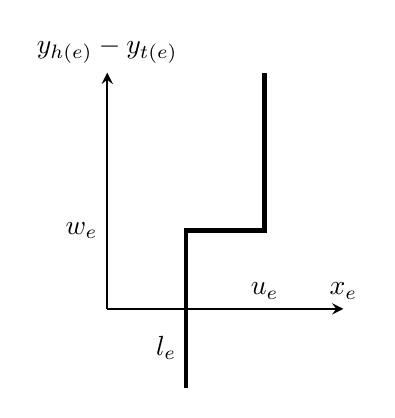
\begin{tikzpicture}
                    \draw [arrow] (0, 0) -- (0, 3);
                    \draw [arrow] (0, 0) -- (3, 0);
                    \draw [link, line width=0.6 mm] (1, -1) -- (1, 1) -- (2, 1) -- (2, 3);
                    \draw node at (0, 3) [above] {$y_{h(e)} - y_{t(e)}$};
                    \draw node at (3, 0) [above] {$x_e$};
                    \draw node at (1, -0.5) [left] {$l_e$};
                    \draw node at (2, 0) [above] {$u_e$};
                    \draw node at (0, 1) [left] {$w_e$};
                \end{tikzpicture}
            \end{figure}

            For each point $(x_e, y_{h(e)} - y_{t(e)})$ we define a \textbf{kilter-number} $k_e$, be the minimum positive distance change in $x_e$ required to put in on the kilter line.
            \begin{example}
                For edge $e: w_e = 2, l_e = 0, u_e = 3$, assume $x_e = 2, y_{h(e)} - y_{t(e)} = 3$, then $k_e = 1$
            \end{example}

            \begin{figure}[!ht]
                \centering
                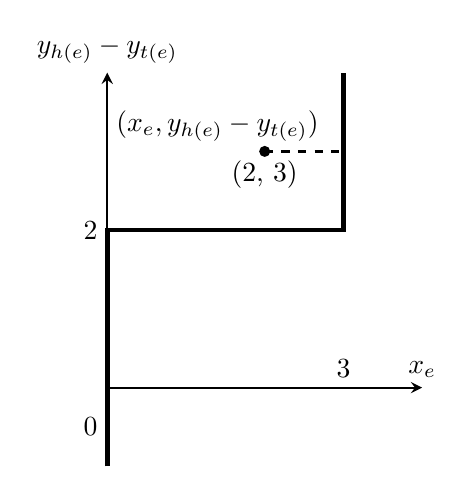
\begin{tikzpicture}
                    \draw [arrow] (0, 0) -- (0, 4);
                    \draw [arrow] (0, 0) -- (4, 0);
                    \draw [link, line width=0.6 mm] (0, -1) -- (0, 2) -- (3, 2) -- (3, 4);
                    \draw node at (0, 4) [above] {$y_{h(e)} - y_{t(e)}$};
                    \draw node at (4, 0) [above] {$x_e$};
                    \draw node at (0, -0.5) [left] {0};
                    \draw node at (3, 0) [above] {3};
                    \draw node at (0, 2) [left] {2};
                    \fill (2, 3) circle [radius=2 pt];
                    \draw node at (2, 3) [above, xshift=-0.6 cm] {$(x_e, y_{h(e)} - y_{t(e)})$};
                    \draw node at (2, 3) [below] {(2, 3)};
                    \draw [link, dashed] (2, 3) -- (3, 3);
                \end{tikzpicture}
            \end{figure}

            \begin{lemma}
                If for every circulation $x$ and vertex number $y$ we have $\sum_{e \in A} k_e = 0$, then $x$ is optimal.
            \end{lemma}

            \begin{proof}
                Since $k_e$ is a nonnegative number, then the only way that $\sum_{e \in A} k_e = 0$ is $k_e = 0, \forall e\in A$, which means $\forall e\in A, l_e \le x_e \le u_e$. Furthermore, the complementary slackness are satisfied.
            \end{proof}

            General idea of algorithm is as follows. Suppose we are given a circulation $x$ and vertex-numbers $y$ (we do not require feasibility). Usually we pick $x=0, y=0$. If every edge is in kilter-line then we are optimal.

            Otherwise there is at least one edge $e^*$ that is out-of kilter. The algorithm consist of two phases, one called \textbf{flow-change} phase (horizontally), then other \textbf{number-change} phase (vertically).

            In the flow-change phase, we want to find a new circulation for an out-of-kilter edge $e^*$ say $\hat{e}$ such that we reduce the kilter number $k_{e^*}$, without increasing any other kilter number for other edges.

            To do this, denote the edges of $e^*$ to be $s$ and $t$, where such that $k_{e^*}$ will be decreased by increasing the flow from $s$ to $t$ on $e^*$.

            If $e^*=(s, t)$ this will accomplished by increasing $x_{e^*}$ and if $e=(t, s)$ it is accomplished by decreasing $x_{e^*}$. 

            To do this we look for an $(s, t)$-path $p$ of the following edges.

            \begin{itemize}
                \item If $e$ is forward in $p$, then increasing $x_e$ does not increase $k_e$ and
                \item If $e$ is reversed in $p$, then decreasing $x_e$ dose not increase $k_e$
            \end{itemize}

            In terms of kilter diagram, an arc satisfies ``forward'' if it is forward and in left side of kilter line, and it satisfies ``reversed'' if it is reverse and in right side of kilter line.

            Suppose we can not find such a path. From $s$ to $t$, let $x$ be the vertices that can decrease by an augmenting path. Then either we can change the vertex numbers $y$ so that $\sum_{e\in A} k_e$ does not increase but $x$ does, or we can show that problem is infeasible.

            The sketch of Out-of-kilter algorithm is as follows:
            \begin{itemize}
                \item \textbf{INPUT} a minimum circulation problem $(D, l, u, w)$ a circulation $x$ and vertex-numbers $y$
                \item \textbf{OUTPUT} conclusion that $(D, l, u, w)$ is infeasible or an minimum weighted flow.
                \item Step 1: If every arc is in kilter $(k_e = 0, \forall e\in A)$. Stop with $x$ is optimal. Otherwise let $e^*$ be an out-of-kilter arc. If increasing $x_{e^*}$ decreases $k_{e^*}$ set $s=h(e^*)$ and $t(e^*)$ otherwise set $s=t(e^*)$ and $t=h(e^*)$
                \item Step 2: If there exists an $(s, t)$ augmenting path $p$ then goto Step 3, otherwise goto Step 4.
                \item Step 3: Set $y_e = y_{h(e)} - y_{t(e)}, e\in A$
                $\begin{cases}
                    \Delta_1 &= \min\{u_e - x_e: e \text{ is forward and } y_e \ge w_e\}\\
                    \Delta_2 &= \min\{l_e - x_e: e \text{ is forward and } y_e < w_e\}\\
                    \Delta_3 &= \min\{x_e - l_e: e \text{ is reverse and } y_e \le w_e\}\\
                    \Delta_4 &= \min\{x_e - u_e: e \text{ is reverse and } y_e > w_e\}
                \end{cases}$\\
                and $\Delta = \min\{\Delta_i, i = 1, 2, 3, 4\}$. Increase $x_e$ by $\Delta$ on each forward arc in $p$, decrease $x_e$ by $\Delta$ on each reverse arc in $p$.\\
                If $e^* = (s, t)$ decrease $x_{e^*}$ by $\Delta$, otherwise increase $x_{e^*}$ by $\Delta$\\
                If $k_{e^*} > 0$ goto Step 2. otherwise goto Step 1.
                \item Step 4: Let $X$ be the set of vertices reachable from $s$ by augmenting paths, then $t \notin X$, if every arc $e$ with $h(e) \in X$ has $x_e \le l_e$ and every arc $e$ with $t(e) \in X$ has $x_e \ge u_e$, and at least one of the above inequality is strict, then Stop with problem infeasible. Otherwise set
                    $\delta_1 = \min\{w_e - y_e: t(e) \in X, y_e < w_e, x_e \le u_e \neq l_e\}$
                    $\delta_2 = \min\{y_e - w_e: h(e) \in X, y_e > w_e, x_e \ge u_e \neq l_e\}$
                    $\delta = \min\{\delta_1, \delta_2\}$
                Set $y_i = y_i + \delta$ for $i \notin X$. If $k_{e^*} > 0$, goto Step 2, otherwise goto Step 1.
            \end{itemize}                

            Out-of-kilter takes $O(|E||V|K)$ where $K = \sum_{e\in A} k_e$. However, there is an algorithm called \textbf{scaling algorithm} that uses out-of-kilter as subroutine that runs in $O(R|E|^2|V|)$ where $R = \lceil \max\{\log_2 u_e: e\in A\}\rceil$
\end{document}